
\begin{figure*}[t]
    \centering
    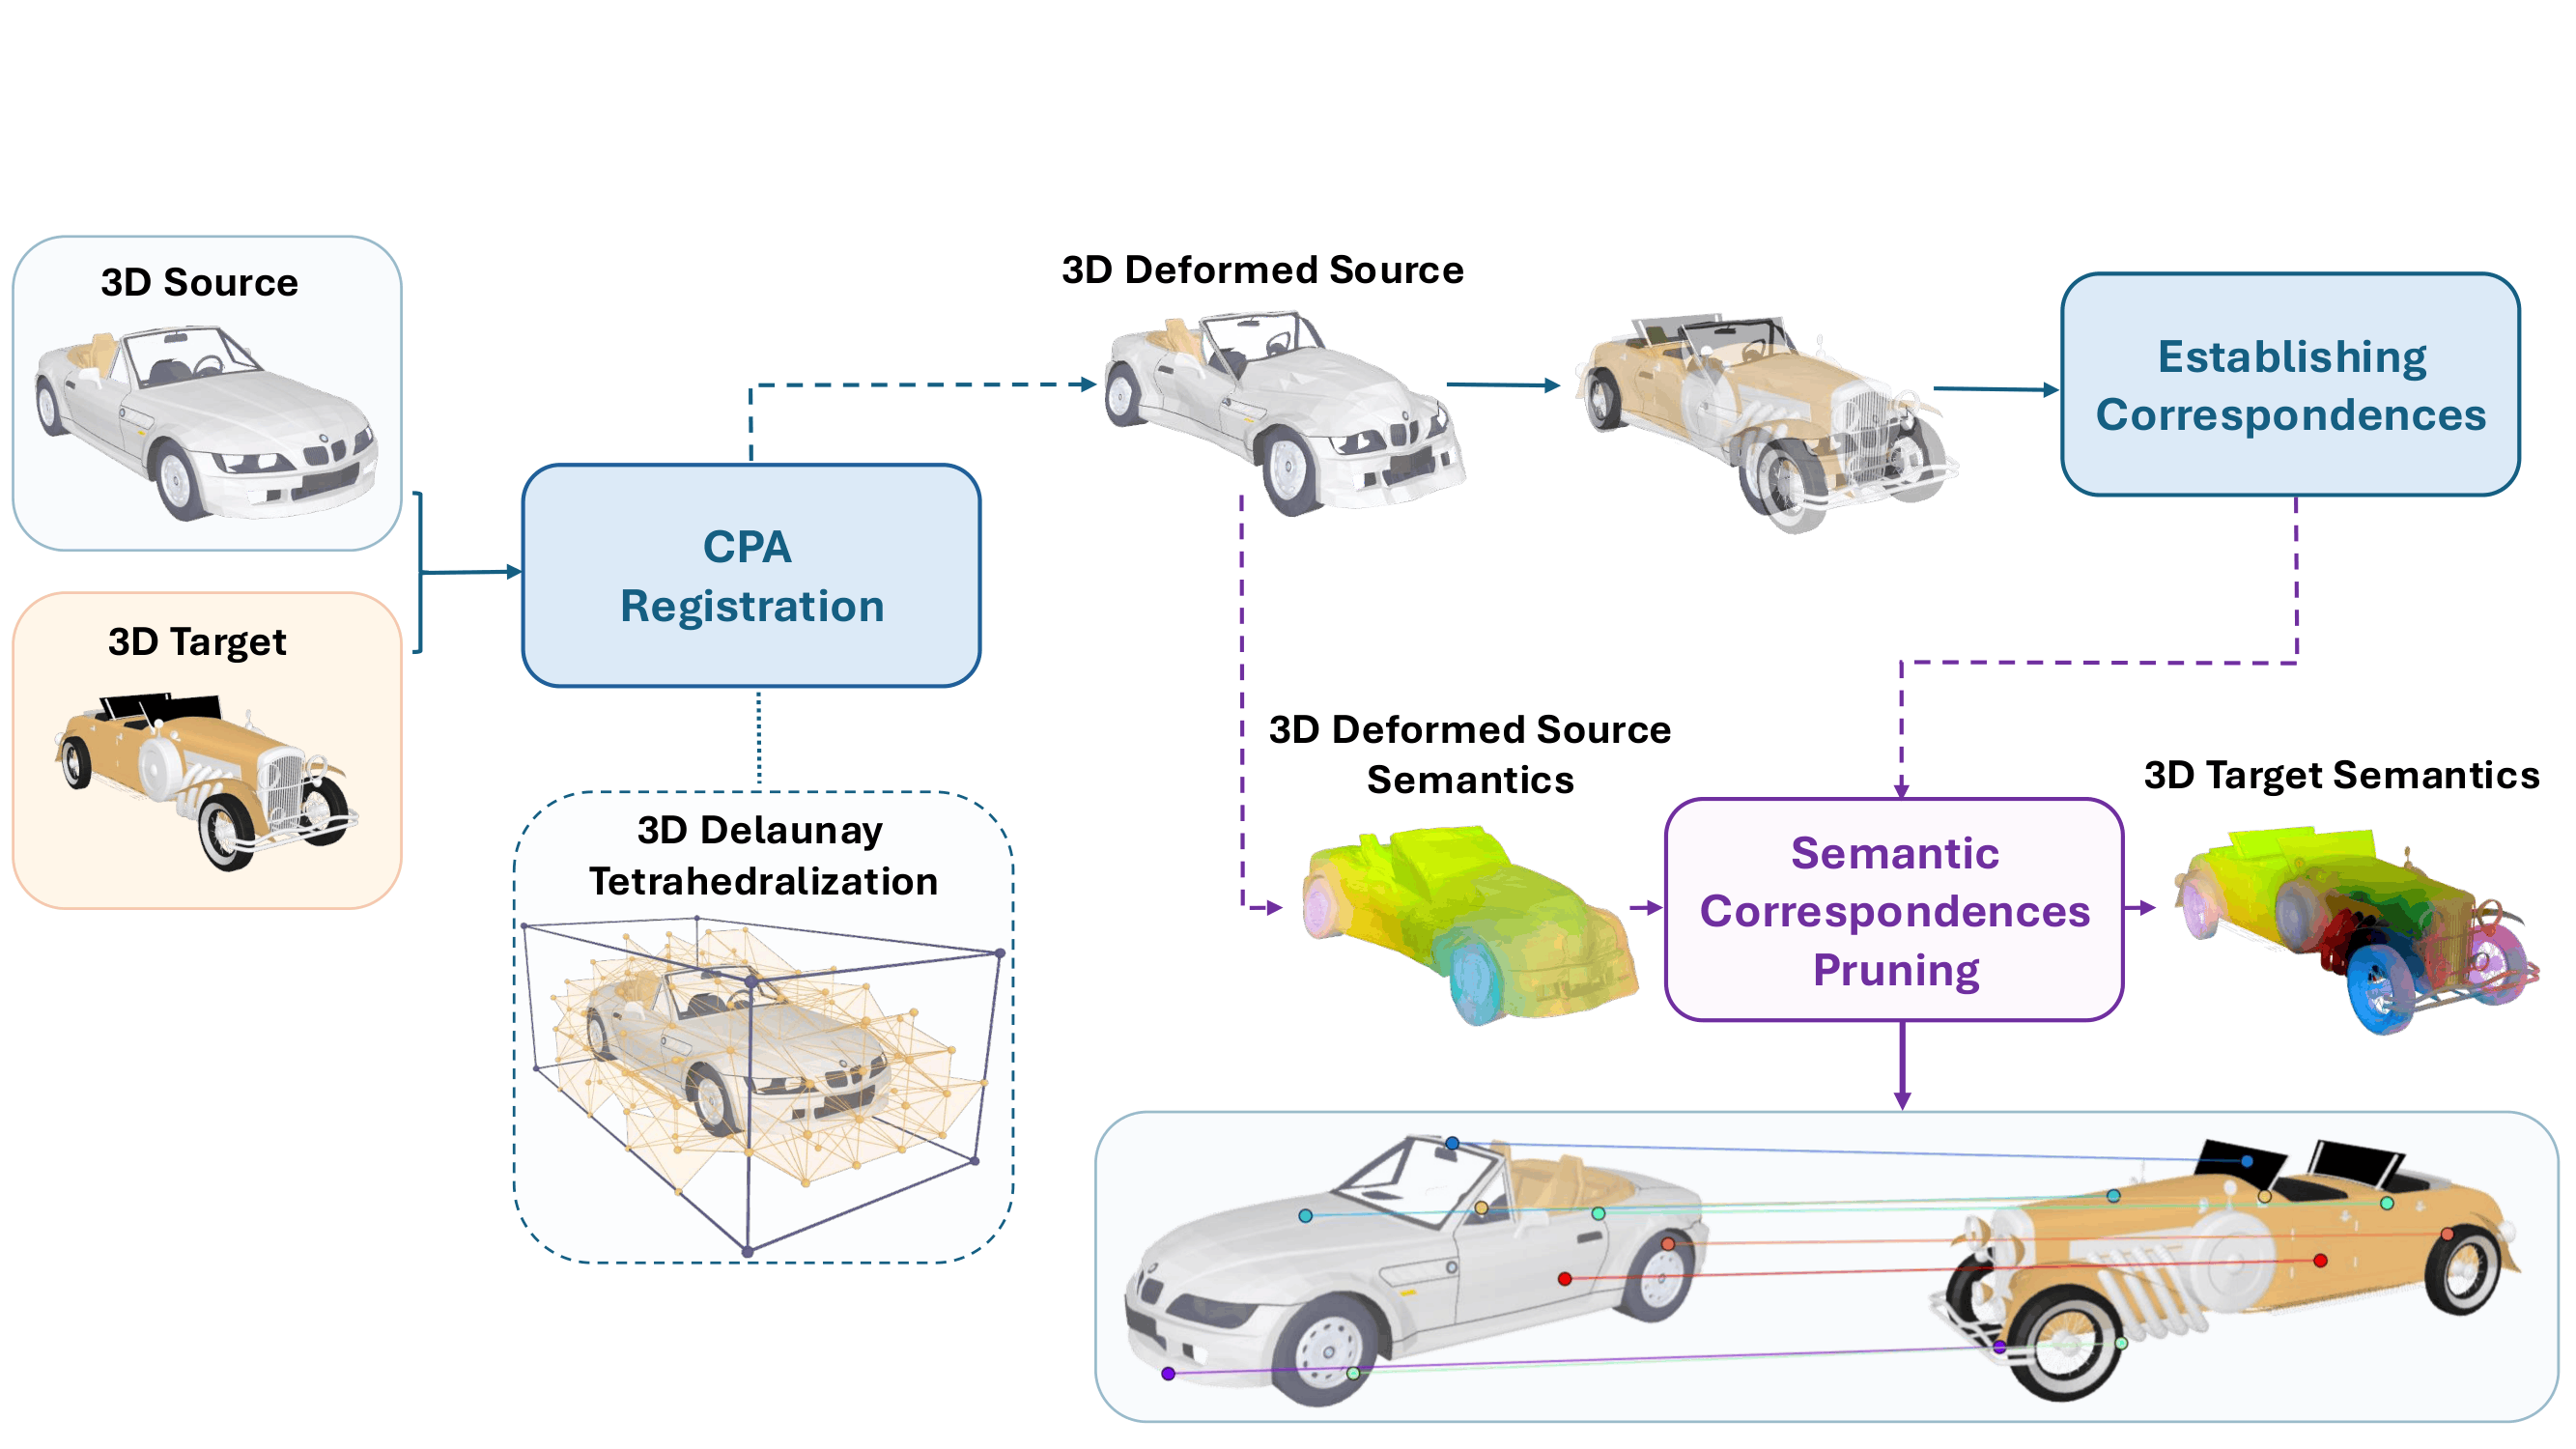
\includegraphics[
        width=\textwidth,
        trim={0pt 25pt 0pt 245pt},
        clip
    ]{figures/method/powerpoint_full_method.png}
    \vspace{-4mm}
    \caption{Overview of our correspondence generation pipeline.}
    \label{fig:method_overview}
\end{figure*}


% \begin{figure*}[t]
% \centering
% \resizebox{\textwidth}{!}{
% \begin{tikzpicture}[
%     node distance=1.2cm,
%     box/.style={
%         rounded corners=6pt,
%         fill=blue!12,
%         minimum width=3.0cm,
%         minimum height=1.1cm,
%         align=center,
%         font=\large
%     },
%     arrow/.style={->, thick, >=latex}
% ]

% \node[align=center] (source) {
%     \textbf{3D source object}\\[2mm]
%     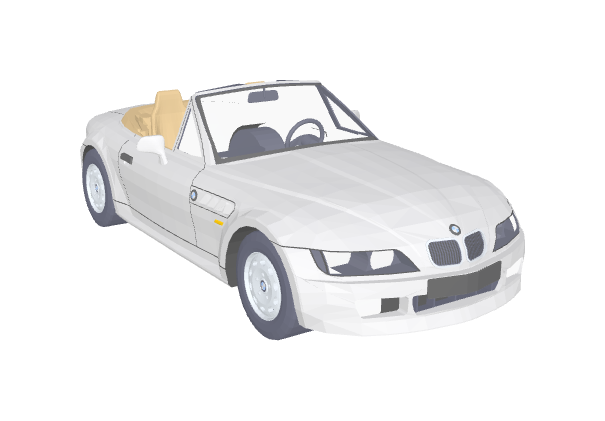
\includegraphics[width=3.0cm]{figures/method/source.png}
% };

% \node[align=center, below=1.0cm of source] (target) {
%     \textbf{3D target object}\\[2mm]
%     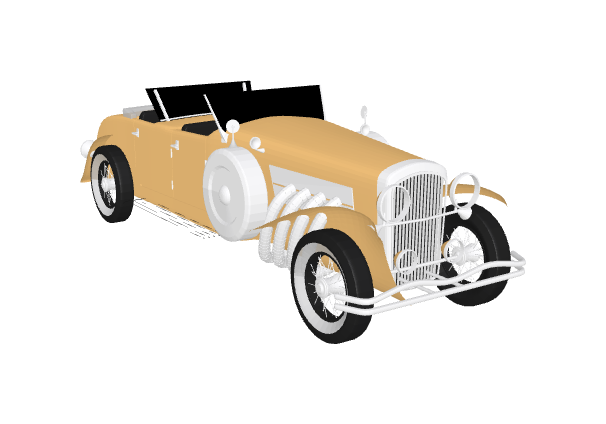
\includegraphics[width=3.0cm]{figures/method/target.png}
% };

% \node[box, right=2.2cm of source, yshift=-1.7cm] (cpa) {
%     CPA Registration
% };

% \coordinate (midleft) at ($(source.east)!0.5!(target.east)$);
% \draw[arrow] (midleft) -- (cpa.west);

% \node[align=center, below=0.9cm of cpa] (cpa_vis) {
%     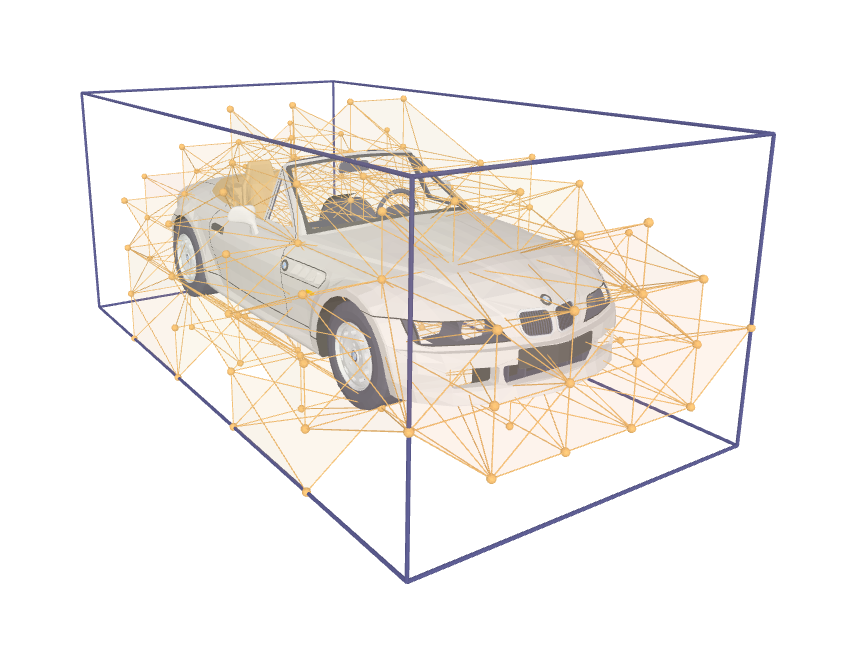
\includegraphics[width=4.8cm]{figures/method/cpa_registration.png}
% };

% \node[align=center, right=2.0cm of cpa] (deformed_src) {
%     \textbf{Deformed source object}\\[2mm]
%     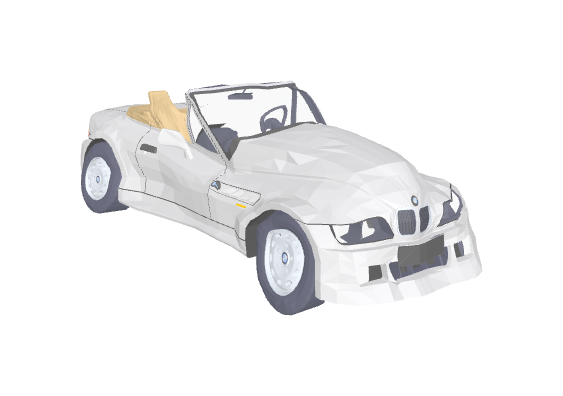
\includegraphics[width=3.2cm]{figures/method/deformed_source.png}
% };

% \draw[arrow] (cpa.east) -- (deformed_src.west);

% \node[box, right=2.0cm of deformed_src] (corr) {
%     Correspondences\\Establishment
% };

% \draw[arrow] (deformed_src.east) -- (corr.west);

% \node[align=center, above=0.9cm of corr] (corr_vis) {
%     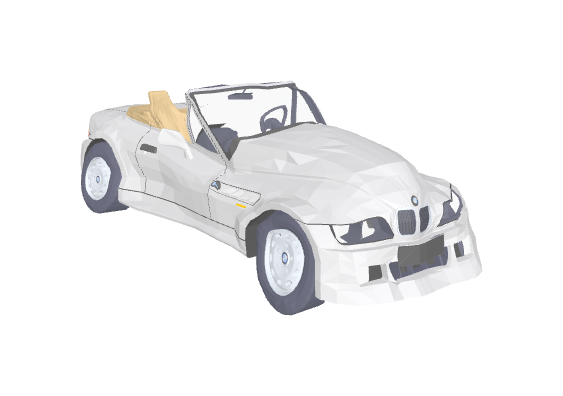
\includegraphics[width=3.8cm]{figures/method/deformed_source.png}
% };

% \node[align=center, below=1.2cm of deformed_src] (srcsem) {
%     \textbf{Deformed source}\\
%     \textbf{semantics}\\[2mm]
%     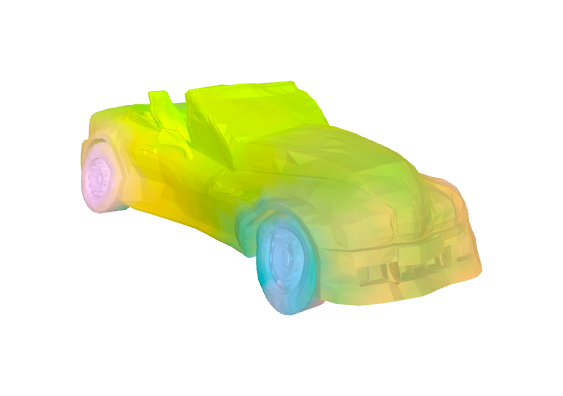
\includegraphics[width=3.0cm]{figures/method/deformed_source_semantics.png}
% };

% \node[align=center, right=4.0cm of srcsem] (tgtsem) {
%     \textbf{Target object}\\
%     \textbf{semantics}\\[2mm]
%     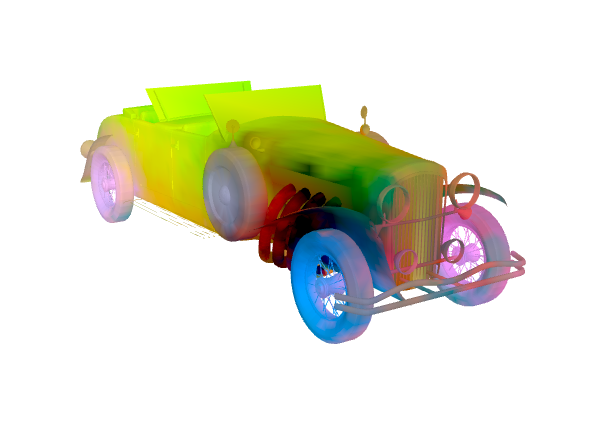
\includegraphics[width=3.0cm]{figures/method/target_semantics.png}
% };

% \node[box, below=1.2cm of corr] (prune) {
%     Semantic\\Correspondences\\Pruning
% };

% \draw[arrow] (corr.south) -- (prune.north);

% \node[align=center, below=1.3cm of prune] (final) {
%     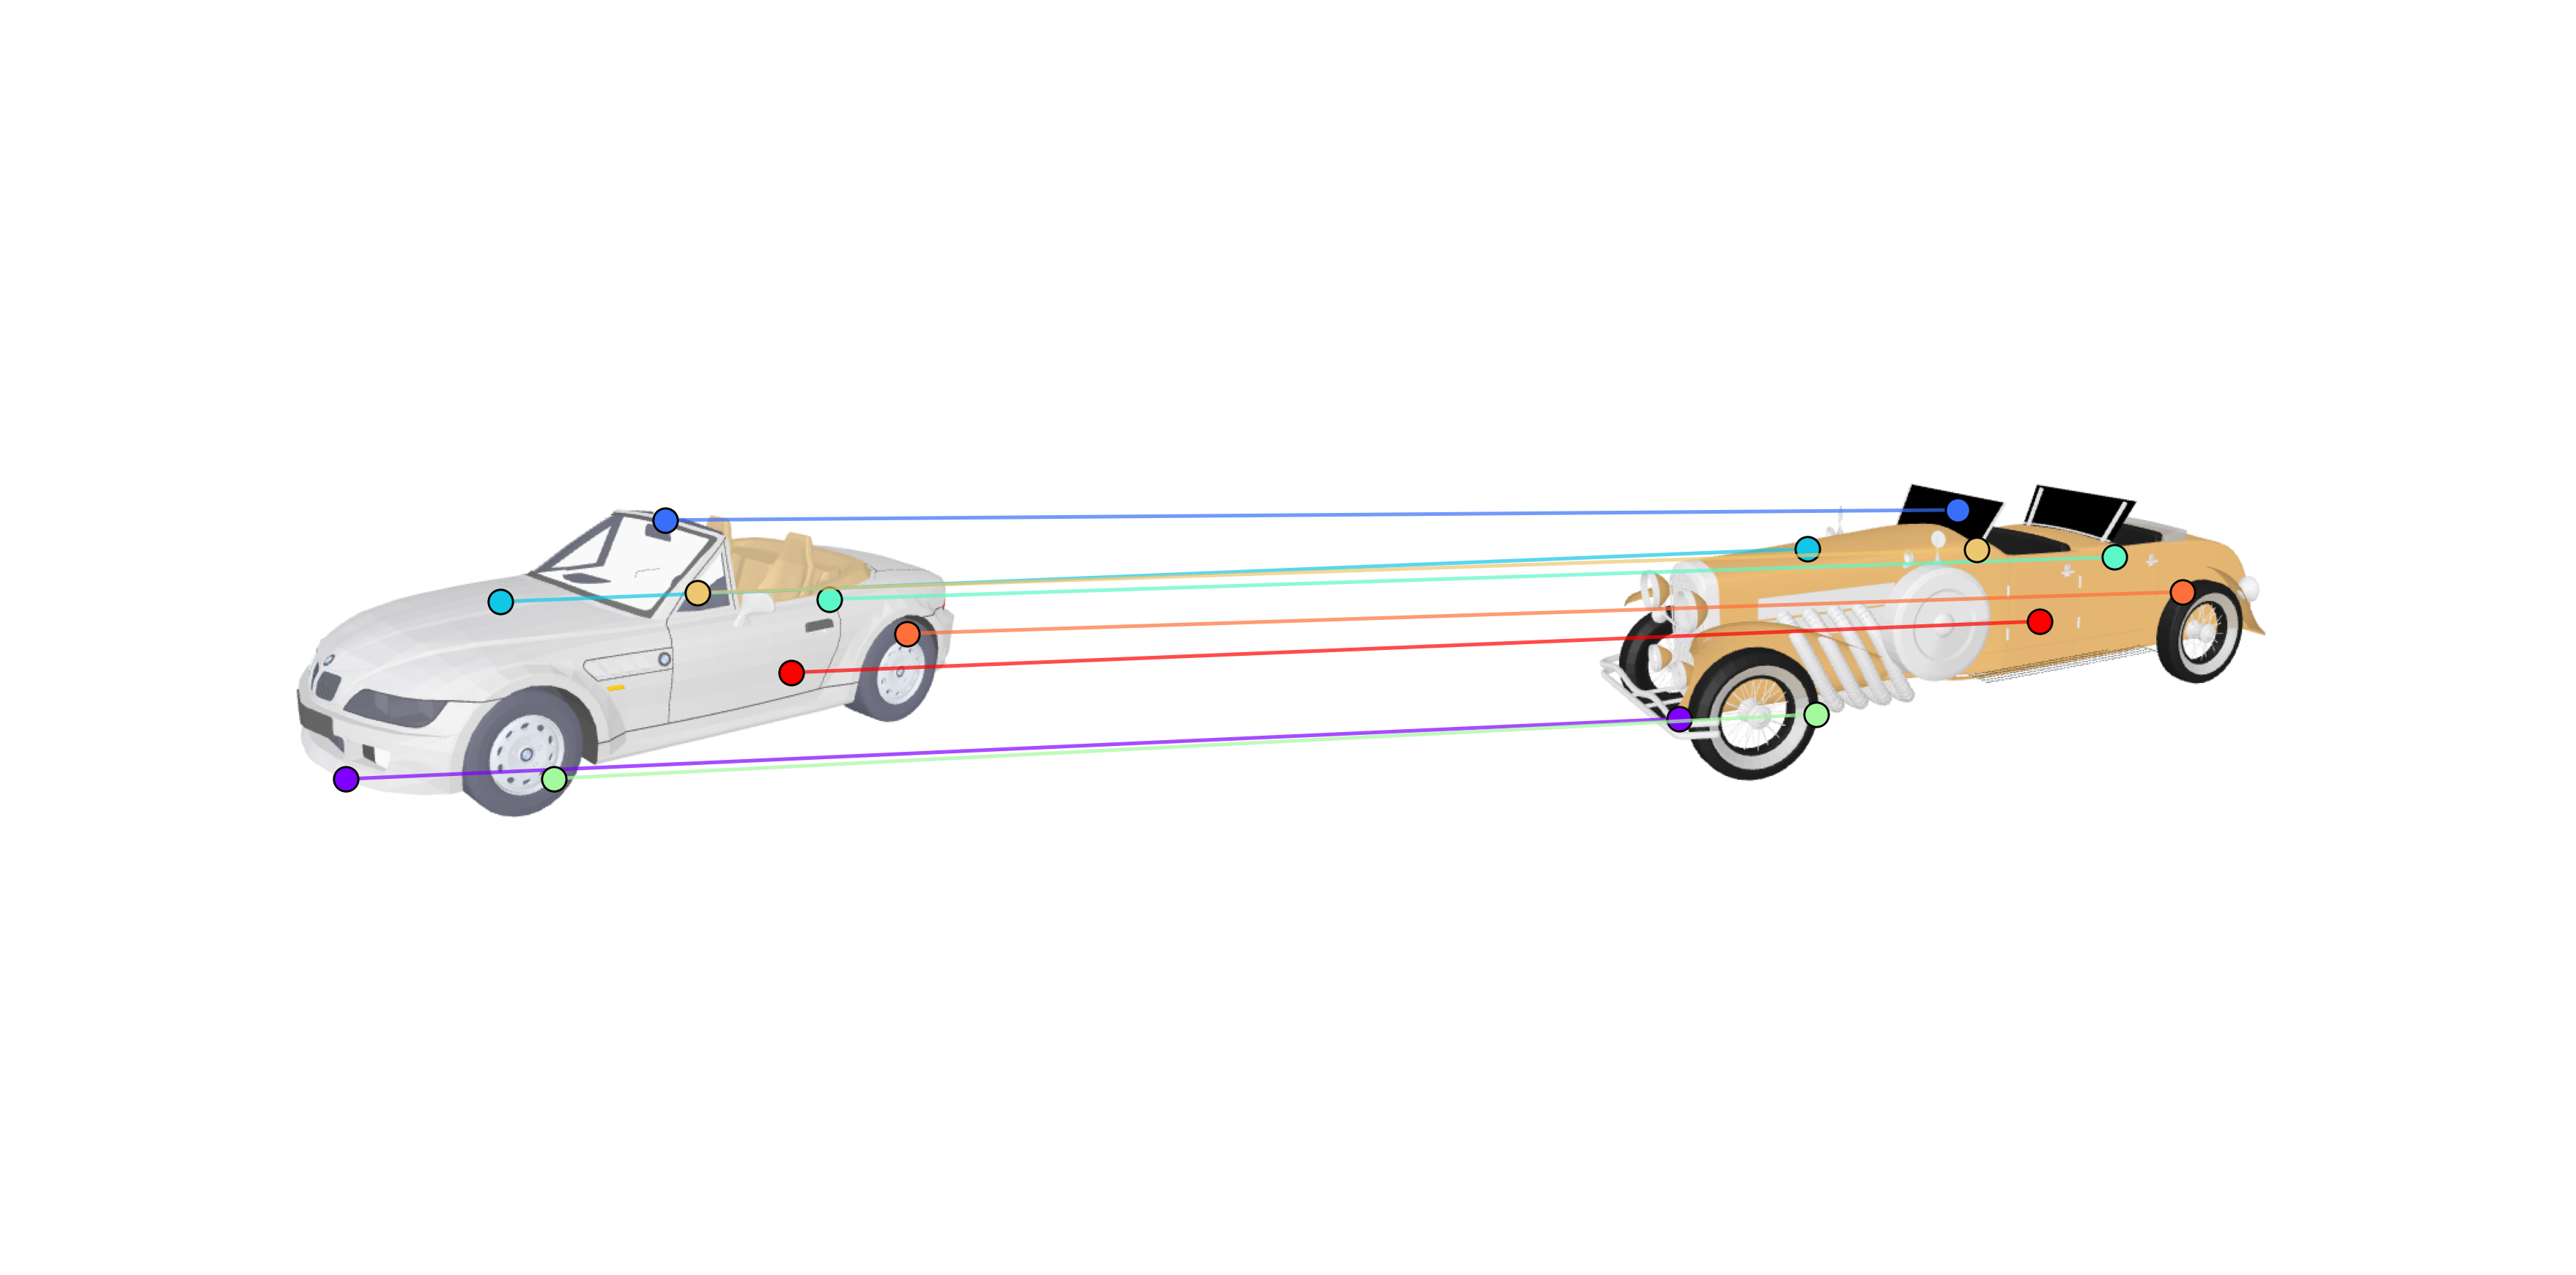
\includegraphics[width=6.5cm]{figures/method/final_correspondences.png}
% };

% \draw[arrow] (prune.south) -- (final.north);

% \end{tikzpicture}
% }
% \caption{Overview of our correspondence generation pipeline.}
% \label{fig:method_overview}
% \end{figure*}
We propose a fully automatic pipeline for generating approximate 3D--3D cross-instance semantic-geometric correspondences between rigid objects, which can be projected into rendered views to obtain 3D--2D and 2D--2D correspondences.
%
The pipeline's input is a collection of object pairs
\(\mathcal{P}=\{(\mathcal{S}_k,\mathcal{T}_k)\}_{k=1}^{K}\), where each source object \(\mathcal{S}_k\) and target object \(\mathcal{T}_k\) are rotation-aligned and normalized to a common scale.
This assumption provides a weak category-level geometric prior, but does not provide any point-level, part-level, or correspondence supervision.

For each object pair, our pipeline proceeds in three main stages.
First, we extract per-point semantic descriptors by rendering each object from multiple views, computing dense DINOv2 features, and lifting them back to 3D (\autoref{sec:feature_lifting}).
Second, we estimate a continuous piecewise-affine (CPA) deformation from the source to the target and extract candidate correspondences via nearest-neighbor assignment after alignment.
Third, we prune semantically inconsistent matches, retaining approximate correspondences that are jointly constrained by deformable geometric alignment and multi-view semantic consistency.

In addition, we optionally apply a bidirectional semantic-coverage filter (\autoref{sec:pair_filter}) before registration to reject object pairs with insufficient semantic overlap.
This step reduces the number of retained pairs, but improves the quality of the remaining pairs and the resulting correspondences.
The full procedure is summarized in \hyperref[alg:correspondence_generation]{Algorithm~\ref*{alg:correspondence_generation}}.

\subsection{Object Representation and Feature Lifting}
\label{sec:feature_lifting}

Each object \(\mathcal{O}\) is represented as a point cloud with an associated semantic feature map:
\begin{equation}
\label{eq:object_representation}
\mathcal{O}=(\mathcal{X},\mathcal{F}),
\qquad
\mathcal{X}=\{x_i\}_{i=1}^{N}, \; x_i\in\mathbb{R}^{3},
\qquad
\mathcal{F}=\{f_i\}_{i=1}^{N}, \; f_i\in\mathbb{R}^{C}.
\end{equation}
Here, \(x_i\) denotes a 3D point sampled from the object surface, and \(f_i\) denotes its corresponding semantic descriptor.
% 
To obtain these descriptors, we render each object from a set of calibrated virtual cameras, extract dense DINOv2 \cite{oquab2024dinov2} features in image space, and lift them back to the visible 3D points using known camera projection and depth.
We then aggregate multi-view observations to obtain a single semantic descriptor for each 3D point.
% 
For a source-target pair \((\mathcal{S},\mathcal{T})\), we write
\begin{equation}
\label{eq:source_target_representation}
\mathcal{S}=(\mathcal{X}_S,\mathcal{F}_S),
\qquad
\mathcal{T}=(\mathcal{X}_T,\mathcal{F}_T),
\end{equation}
where
\(\mathcal{X}_S=\{x_i^S\}_{i=1}^{N_S}\),
\(\mathcal{X}_T=\{x_j^T\}_{j=1}^{N_T}\),
\(\mathcal{F}_S=\{f_i^S\}_{i=1}^{N_S}\), and
\(\mathcal{F}_T=\{f_j^T\}_{j=1}^{N_T}\).

\subsection{Semantic Similarity}
\label{sec:semantic_sim}

We measure semantic compatibility using cosine similarity in the reduced descriptor space. Specifically, we apply Principal Component Analysis (PCA) jointly to the source and target DINOv2 descriptors and reduce them to 64 dimensions. We denote the reduced descriptor corresponding to \(f_i\) by \(z_i\).

Given two points \(x_i\) and \(x_j\) with reduced descriptors \(z_i\) and \(z_j\), we define the semantic similarity as
\begin{equation}
\label{eq:semantic_similarity}
s_{\mathrm{sem}}(x_i,x_j)
=
\frac{z_i^\top z_j}{\|z_i\|_2 \|z_j\|_2}.
\end{equation}

Two points are considered semantically compatible if
\begin{equation}
\label{eq:semantic_compatibility}
s_{\mathrm{sem}}(x_i,x_j) > \tau_{\mathrm{sem}},
\end{equation}
where \(\tau_{\mathrm{sem}} = 0.85\) in all experiments.


\subsection{Optional Semantic Coverage Pair Filtering}
\label{sec:pair_filter}

As an optional preprocessing stage, we apply bidirectional semantic-coverage filtering before registration.

For a source-target pair \((\mathcal{S},\mathcal{T})\), we define the source-to-target semantic coverage as
\begin{equation}
\label{eq:semantic_coverage}
\rho_{\mathrm{sem}}(\mathcal{S} \rightarrow \mathcal{T})
=
\frac{1}{|\mathcal{X}_S|}
\sum_{x_i^S \in \mathcal{X}_S}
\mathbf{1}
\left[
\max_{x_j^T \in \mathcal{X}_T}
s_{\mathrm{sem}}(x_i^S,x_j^T)
>
\tau_{\mathrm{sem}}
\right],
\end{equation}
where \(\mathbf{1}[\cdot]\) denotes the indicator function, which equals \(1\) if the condition inside the brackets is true and \(0\) otherwise. This score measures the fraction of source points that have at least one semantically compatible point in the target.
We also compute the same quantity in the reverse direction, \(\rho_{\mathrm{sem}}(\mathcal{T} \rightarrow \mathcal{S})\), and retain the object pair only if
\begin{equation}
\label{eq:pair_filter}
\rho_{\mathrm{sem}}(\mathcal{S} \rightarrow \mathcal{T}) \geq \gamma
\quad \text{and} \quad
\rho_{\mathrm{sem}}(\mathcal{T} \rightarrow \mathcal{S}) \geq \gamma .
\end{equation}
In our experiments, we use \(\gamma = 0.6\).



\subsection{Continuous Piecewise-Affine Registration}
\label{sec:registration_cpa}

For each retained object pair \((\mathcal{S},\mathcal{T})\), we estimate a non-rigid transformation that aligns the source point set \(\mathcal{X}_S\) to the target \(\mathcal{X}_T\).
We model this transformation using a continuous piecewise-affine (CPA) mapping
\begin{equation}
\label{eq:cpa_transform}
T_{\mathrm{CPA}}:\mathbb{R}^{3}\rightarrow\mathbb{R}^{3},
\end{equation}
which produces a continuous, spatially coherent deformation field while allowing local shape variation across object instances.
%
This transformation is parameterized by a regular control grid over the normalized 3D domain, which is decomposed into tetrahedral cells using Delaunay triangulation.
Each grid vertex is associated with a learnable displacement vector, and the displacement of an arbitrary source point is obtained by barycentric interpolation from the vertices of the tetrahedron containing it.
This yields a deformation field that is locally affine within each tetrahedron and continuous across neighboring cells.

We estimate the transformation by optimizing a Chamfer distance loss~\cite{fan2017chamfer} with smoothness regularization via gradient descent:
\begin{equation}
\label{eq:cpa_objective}
\mathcal{L}_{\mathrm{CPA}}
=
\mathcal{L}_{\mathrm{Chamfer}}
\left(
T_{\mathrm{CPA}}(\mathcal{X}_S),
\mathcal{X}_T
\right)
+
\lambda_{\mathrm{smooth}}
\mathcal{R}(T_{\mathrm{CPA}}),
\end{equation}
where \(\lambda_{\mathrm{smooth}} = 0.3\) in all experiments, and 
\begin{equation}
\label{eq:chamfer_loss}
\mathcal{L}_{\mathrm{Chamfer}}
(\widehat{\mathcal{X}}_S,\mathcal{X}_T)
=
\frac{1}{|\widehat{\mathcal{X}}_S|}
\sum_{\hat{x}_i^S \in \widehat{\mathcal{X}}_S}
\min_{x_j^T \in \mathcal{X}_T}
\left\|
\hat{x}_i^S-x_j^T
\right\|_2^2
+
\frac{1}{|\mathcal{X}_T|}
\sum_{x_j^T \in \mathcal{X}_T}
\min_{\hat{x}_i^S \in \widehat{\mathcal{X}}_S}
\left\|
x_j^T-\hat{x}_i^S
\right\|_2^2 .
\end{equation}

The first term aligns the deformed source to the target, while the second term encourages the target surface to be covered by the deformed source.

The smoothness term regularizes neighboring control-grid displacements:
\begin{equation}
\label{eq:cpa_smoothness}
\mathcal{R}(T_{\mathrm{CPA}})
=
\frac{1}{|\mathcal{E}|}
\sum_{(v_a,v_b)\in\mathcal{E}}
\left\|
u_{v_a}-u_{v_b}
\right\|_2^2,
\end{equation}
where \(\mathcal{E}\) denotes edges between neighboring vertices in the tetrahedral control grid.
This regularization promotes locally coherent deformations while still allowing non-rigid cross-instance variation.
%
After optimization, the transformed source point cloud is given by
\begin{equation}
\label{eq:deformed_source}
\widehat{\mathcal{X}}_S
=
T_{\mathrm{CPA}}(\mathcal{X}_S)
=
\{\hat{x}_i^S\}_{i=1}^{N_S}.
\end{equation}

\begin{algorithm}[t]
\DontPrintSemicolon
\caption{Automatic Approximate Semantic-Geometric Correspondence Generation}
\label{alg:correspondence_generation}

\KwIn{
Rotation-aligned and scale-normalized object pairs 
\(\mathcal{P}=\{(\mathcal{S}_k,\mathcal{T}_k)\}_{k=1}^{K}\);
lifted 3D DINOv2 features;
semantic similarity threshold \(\tau_{\mathrm{sem}}\);
optional coverage threshold \(\gamma\).
}
\KwOut{
Approximate semantic-geometric correspondences.
}

\ForEach{\((\mathcal{S},\mathcal{T}) \in \mathcal{P}\)}{

    Let \((\mathcal{X}_S,\mathcal{F}_S)\) and \((\mathcal{X}_T,\mathcal{F}_T)\) be the source and target representations\;

    \If{semantic coverage filtering is enabled}{
        \If{\(\rho_{\mathrm{sem}}(\mathcal{S}\!\rightarrow\!\mathcal{T}) < \gamma\) 
        \textbf{or} 
        \(\rho_{\mathrm{sem}}(\mathcal{T}\!\rightarrow\!\mathcal{S}) < \gamma\)}{
            \textbf{continue}\;
        }
    }

    Estimate \(T_{\mathrm{CPA}}\) by minimizing Eq.~\eqref{eq:cpa_objective}\;

    Compute the deformed source 
    \(\widehat{\mathcal{X}}_S = T_{\mathrm{CPA}}(\mathcal{X}_S)\)\;

    Assign each \(\hat{x}_i^S \in \widehat{\mathcal{X}}_S\) to its nearest neighbor in \(\mathcal{X}_T\) using Eq.~\eqref{eq:nearest_neighbor_assignment}\;

    Construct candidate correspondences \(\mathcal{C}_{\mathcal{S},\mathcal{T}}^{0}\)\;

    Prune correspondences using the semantic criterion in Eq.~\eqref{eq:semantic_pruning_condition}\;

    Store the final correspondence set \(\mathcal{C}_{\mathcal{S},\mathcal{T}}\)\;
}

\textbf{Return} all processed object pairs that were not filtered out and their correspondence sets.

\end{algorithm}

\subsection{Approximate Correspondence Extraction}
\label{sec:establish_correspondences}

After CPA registration, the source and target are approximately aligned geometrically.
We then assign each transformed source point to its nearest neighbor in the target point cloud.
For each \(\hat{x}_i^S \in \widehat{\mathcal{X}}_S\), the target index is
\begin{equation}
\label{eq:nearest_neighbor_assignment}
a(i)
=
\arg\min_{j\in\{1,\ldots,N_T\}}
\left\|
\hat{x}_i^S-x_j^T
\right\|_2 .
\end{equation}
This produces an initial set of candidate correspondences:
\begin{equation}
\label{eq:initial_correspondences}
\mathcal{C}_{\mathcal{S},\mathcal{T}}^{0}
=
\left\{
\left(x_i^S,x_{a(i)}^T\right)
\; \middle| \;
i=1,\ldots,N_S
\right\}.
\end{equation}
Importantly, the assignment is computed using the deformed source point \(\hat{x}_i^S\), while the stored correspondence is defined between the original source point \(x_i^S\) and the target point \(x_{a(i)}^T\).
These matches should therefore be interpreted as approximate cross-instance correspondences induced by deformation-based alignment, rather than exact point-level annotation.

\subsection{Semantic Consistency Pruning}
\label{sec:semantic_pruning}

Geometric proximity alone may produce implausible matches in close regions with different semantics or regions with no meaningful semantic counterpart.
We therefore apply a final semantic pruning step to retain only candidate matches that are also semantically compatible.
A candidate correspondence \((x_i^S,x_{a(i)}^T)\in\mathcal{C}_{\mathcal{S},\mathcal{T}}^{0}\) is retained only if
\begin{equation}
\label{eq:semantic_pruning_condition}
s_{\mathrm{sem}}
\left(
x_i^S,
x_{a(i)}^T
\right)
>
\tau_{\mathrm{sem}}.
\end{equation}
The final semantic-geometric correspondence set is
\begin{equation}
\label{eq:final_correspondences}
\mathcal{C}_{\mathcal{S},\mathcal{T}}
=
\left\{
\left(x_i^S,x_{a(i)}^T\right)
\in
\mathcal{C}_{\mathcal{S},\mathcal{T}}^{0}
\; \middle| \;
s_{\mathrm{sem}}
\left(
x_i^S,x_{a(i)}^T
\right)
>
\tau_{\mathrm{sem}}
\right\}.
\end{equation}
This step removes matches that are geometrically nearby after deformation but semantically inconsistent according to the lifted DINOv2 \cite{oquab2024dinov2} features.
The remaining set forms our final approximate semantic-geometric correspondences.

\subsection{Projection to 2D Correspondences}
\label{sec:projection_2d}

The generated correspondences, established in 3D, can be directly projected into rendered views to produce aligned 3D--3D, 3D--2D, or 2D--2D supervision. Given calibrated rendering views with camera projections \(\pi_{c_S}\) and \(\pi_{c_T}\), a 3D correspondence \((x_i^S,x_j^T)\in\mathcal{C}_{\mathcal{S},\mathcal{T}}\) induces the 2D projections
\begin{equation}
\label{eq:projection_to_2d}
(u_i^S,u_j^T)
=
\left(
\pi_{c_S}(x_i^S),
\pi_{c_T}(x_j^T)
\right),
\end{equation}
where \(c_S\) and \(c_T\) denote the selected source and target camera views. Projecting one endpoint yields 3D--2D supervision, while projecting both endpoints yields 2D--2D supervision. By rendering multiple views of each object pair, we obtain large-scale automatically generated training data for image-based semantic correspondence models.